\documentclass{article}

% load package with ``framed'' and ``numbered'' option.
\usepackage[framed,numbered,autolinebreaks,useliterate]{mcode}
\usepackage{amsmath}
\usepackage{setspace}
\usepackage{geometry}
\usepackage{graphicx}
\geometry{
    left=2.5cm, % 左边距
    right=2.5cm, % 右边距
    top=2.5cm, % 上边距
    bottom=2.5cm, % 下边距
}

% something NOT relevant to the usage of the package.
\usepackage{url}
\setlength{\parindent}{0pt}
\setlength{\parskip}{18pt}
\title{\mbox{Computer Exercises for Advanced Control Systems}\\ \texttt{Report}}
\vspace{-30pt}
\author{Wenbin Mai, Junsen Wang}
% //////////////////////////////////////////////////

\begin{document}

\maketitle

\section*{CE1: Norms of Systems and Model Uncertainty}
\subsection*{1.1 Norms of SISO systems}
\subsubsection*{1.1.1 2-Norm}
\paragraph{1. The residue theorem.}~\\~\\
\begin{figure}[h]
    \centering
    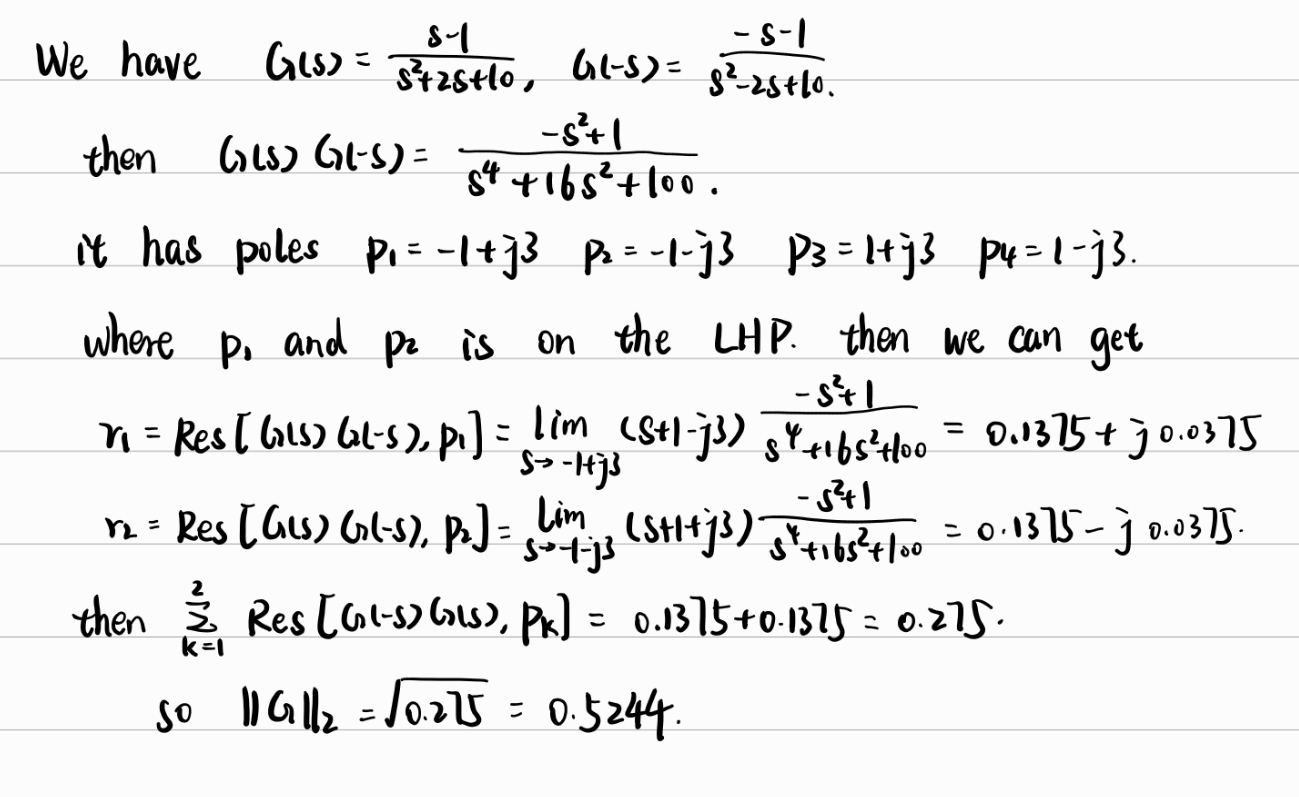
\includegraphics[width=0.8\linewidth]{t1_1_1_1.jpg}
%    \caption{Enter Caption}
%    \label{fig:enter-label}
\end{figure}


\paragraph{2. The frequency response of G.}~\\~\\
We know that for a given transfer function $G$, its 2-norm is defined as follows.
\[||G||_2=(\frac{1}{2\pi}\int^{\infty}_{-\infty}trace[G^*(j\omega)G(j\omega)]d\omega)^{\frac{1}{2}}\]
The approximation of the integral can be written as follows.
\[||G||_2\approx\sqrt{\frac{1}{\pi}\sum^{N}_{k=0}|G(j\omega)|^2\triangle\omega_k}\]
Select $N=10000$, and integrate over the interval where omega ranges from $10^-2$ to $10^6$. Then we get the code as follows.

\begin{lstlisting}{frame=single}
s = tf('s');
gs = (s - 1)/(s^2 + 2*s + 10);

omega = logspace(-2, 6, 10000);
[G_amp, ~] = bode(gs, omega);
G_amp = squeeze(G_amp);

appro_i = trapz(omega, G_amp.^2)/(2*pi);
two_norm_i = sqrt(2*appro_i);
two_norm = norm(gs, 2);

disp("Two norm =");
disp(two_norm_i);
\end{lstlisting}
The output is 
\begin{lstlisting}[numbers=none]
Two norm =
    0.5244
\end{lstlisting}

\paragraph{3. The impulse response of G.}~\\~\\
For stable systems, the 2-norm can be computed using the integral of the square of the impulse response $g(t)$
\[||G||^2_2=\int^{\infty}_{-\infty}|g(t)|^2dt \approx \sum^{N}_{k=0}|g(t_k)|^2\triangle_{t_k}\]
It can also be approximated.
\begin{lstlisting}{}
s = tf('s');
gs = (s - 1)/(s^2 + 2*s + 10);
[gt, t] = impulse(gs);
appro_impluse = trapz(t, gt.^2);
two_norm = sqrt(appro_impluse);

disp("Two norm =");
disp(two_norm_i);
\end{lstlisting}
The output is 
\begin{lstlisting}[numbers=none]
Two norm =
    0.5244
\end{lstlisting}

\paragraph{4. The state-space method}~\\~\\
We can use the command \verb|ssdata| to convert the transfer function $G(s)$ into the matrix $A, B, C, D$ in the state-space model. Then we can solve the following equation(using command \verb|lyap|) to find the matrix $L$:
$$AL+LA^T+BB^T=0$$
The 2-norm of $G$ is given by:
$$||G||_2=\sqrt{trace[CLC^T]}$$
\begin{lstlisting}{}
s = tf('s');
gs = (s - 1)/(s^2 + 2*s + 10);

[A, B, C, D] = ssdata(gs);
L = lyap(A, B*B');
two_norm_ss = sqrt(trace(C*L*C'));
two_norm = norm(gs, 2);

disp("Two norm =");
disp(two_norm_i);
\end{lstlisting}
The output is 
\begin{lstlisting}[numbers=none]
Two norm =
    0.5244
\end{lstlisting}

\paragraph{5. Validate your results with the Matlab command \texttt{norm}}~\\~\\
We used the code \mcode{norm(Gs, 2)} and got the two-norm as \mcode{0.5244}. It validates the results we got from above.

\subsubsection*{1.1.2 $\infty$-Norm}
\paragraph{1. The frequency response of G.}~\\~\\
The $\infty$-norm of $G$ is given by:
\[||G||_\infty= \underset{\omega}{sup} ||G(j\omega)||\]
Then we can use the \verb|bode| command to find the frequency response and calculate its maximum value to get the $\infty$-norm.
\begin{lstlisting}{}
s = tf('s');
gs = (s - 1)/(s^2 + 2*s + 10);

omega = logspace(-1, 4, 5000);
[G_amp, ~] = bode(gs, omega);
G_amp = squeeze(G_amp);

inf_norm = max(G_amp);

disp("Inf norm =");
disp(inf_norm);
\end{lstlisting}
The output is 
\begin{lstlisting}[numbers=none]
Inf norm =
    0.5246
\end{lstlisting}

\paragraph{2. The bounded real lemma.}~\\~\\
We can compute the Hamiltonian matrix $H$ by 
\[ H = \begin{bmatrix} 
A & \gamma^{-2}BB^T \\ -C^TC & -A^T
\end{bmatrix} 
\]
The we can perform the \textit{iterative Bisection algorithm} in MATLAB, choosing the specified level as $\epsilon=10^{-5}$. $\gamma_l$ and $\gamma_u$ starts at $10^{-2}$ and $10$ respectively. We also define a function \verb|judge| to determine whether the eigenvalue of $H$ is on the imaginary axis.
\begin{lstlisting}{}
s = tf('s');
gs = (s - 1)/(s^2 + 2*s + 10);
[A, B, C, D] = ssdata(gs);

eps = 1e-5;
gamma_l=1e-2; 
gamma_h=10;

while( abs(gamma_l-gamma_h)> eps )
    gamma=(gamma_l+gamma_h)/2;
    H=[A  ,(1/gamma^2)*(B*B') ;
          -C'*C ,   -A']  ;
    H=vpa(H,4);
    flag=judge(H);
    if(flag)  
        gamma_l=gamma;
    else
        gamma_h=gamma;
    end
end

inf_norm = gamma;
disp("Inf norm =");
disp(inf_norm);

function flag=judge(H)
    flag=0;
    [~,d]=eig(H); 
    d=vpa(d,4);
    for i=1:max(size(H))
        if(real(d(i,i))==0) 
            flag=1;
            break;
        end
    end
end
\end{lstlisting}
The output is 
\begin{lstlisting}[numbers=none]
Inf norm =
    0.5246
\end{lstlisting}

\paragraph{3. Validate your results with the Matlab command \texttt{norm} }~\\~\\
We used the code \mcode{norm(Gs, inf)} and got the $\infty$-norm as \mcode{0.5246}. It validates the results we got from above.

\subsection*{1.2 Norms of MIMO systems}
\subsubsection*{1.2.1 2-Norm}
\paragraph{1. The frequency response method.}~\\~\\
We know that for a given transfer function $G$, its 2-norm is defined as follows.
\[||G||_2=(\frac{1}{2\pi}\int^{\infty}_{-\infty}trace[G^*(j\omega)G(j\omega)]d\omega)^{\frac{1}{2}}\]
We can compute the $G$ matrix by 
\[G=C(sI-A)^{-1}B+D\]
The we can compute the frequency response of $G^*(j\omega)G(j\omega)$ by approximation, and then we can get the two-norm of $G$.
\begin{lstlisting}{}
A = [20, -27, 7;
     53, -63, 13;
     -5, 12, -8];
B = [1, -1;
    -2, -1;
    -3, 0];
C = [0, 0, -2;
     1, -1, -1];
D = [0, 0;
     0, 0];

s = tf('s');
Gs = C*inv(s*eye(3)-A)*B+D;
Gs_star = ctranspose(Gs);
H = Gs_star*Gs;

omega = logspace(-2, 6, 1000);
[H_amp, ~] = bode(H, omega);

trace_vector = zeros(1, 1000);
for i = 1:1000
    trace_vector(i) = trace(H_amp(:,:,i));
end

two_norm_i = trapz(omega, trace_vector)/(2*pi);
two_norm_i = sqrt(two_norm_i*2);
disp("Two norm =");
disp(two_norm_i);
\end{lstlisting}
The output is 
\begin{lstlisting}[numbers=none]
Two norm =
    2.2811
\end{lstlisting}

\paragraph{2. The state-space method}~\\~\\
We can solve the following equation(using command \verb|lyap|) to find the matrix $L$:
$$AL+LA^T+BB^T=0$$
The 2-norm of $G$ is given by:
$$||G||_2=\sqrt{trace[CLC^T]}$$
\begin{lstlisting}{}
A = [20, -27, 7;
     53, -63, 13;
     -5, 12, -8];
B = [1, -1;
    -2, -1;
    -3, 0];
C = [0, 0, -2;
     1, -1, -1];
D = [0, 0;
     0, 0];

L = lyap(A, B*B');
two_norm_ss = sqrt(trace(C*L*C'));

disp("Two norm =");
disp(two_norm_ss);
\end{lstlisting}
The output is 
\begin{lstlisting}[numbers=none]
Two norm =
    2.2818
\end{lstlisting}

\paragraph{3. Validate your results with the Matlab command \texttt{norm}}~\\~\\
We used the code \mcode{norm(Gs, 2)} and got the two-norm as \mcode{2.2818}.~\\~\\
It is equal to the result we calculated in 1.2.1.2, and the relative error between it and the result we approximately calculated in 1.2.1.1 is $E=\frac{|2.2818-2.2811|}{2.2818}\times 100\%=0.03\%$, which is also acceptable.

\subsubsection*{1.2.2 $\infty$-Norm}
\paragraph{1. The frequency response method.}~\\~\\
The $\infty$-norm of $G$ can be given by:
\[||G||_\infty= \underset{\omega}{sup}~\overline{\sigma}[G(j\omega)]\]
Then we can use the \verb|bode| command to find the frequency response and calculate its largest singular value using \verb|svd| to get the $\infty$-norm.

\begin{lstlisting}{}
A = [20, -27, 7;
     53, -63, 13;
     -5, 12, -8];
B = [1, -1;
    -2, -1;
    -3, 0];
C = [0, 0, -2;
     1, -1, -1];
D = [0, 0;
     0, 0];

s = tf('s');
Gs = C*inv(s*eye(3)-A)*B+D;
omega = logspace(-1, 4, 1000);
[G_amp, ~] = bode(Gs, omega);

svd_vector = zeros(1, 1000);
for i = 1:1000
    svd_vector(i) = max(svd(G_amp(:,:,i)));
end

inf_norm_f = max(svd_vector);
disp("Inf norm = "); 
disp(inf_norm_f);
\end{lstlisting}
The output is 
\begin{lstlisting}[numbers=none]
Inf norm = 
    1.1083
\end{lstlisting}

\paragraph{2. The bounded real lemma.}~\\~\\
Similar to 1.1.2.2, we can perform the \textit{iterative Bisection algorithm} in MATLAB, choosing the specified level as $\epsilon=10^{-5}$. $\gamma_l$ and $\gamma_u$ starts at $10^{-2}$ and $10$ respectively.
\begin{lstlisting}{}
A = [20, -27, 7;
     53, -63, 13;
     -5, 12, -8];
B = [1, -1;
    -2, -1;
    -3, 0];
C = [0, 0, -2;
     1, -1, -1];
D = [0, 0;
     0, 0];

eps = 1e-5;
gamma_l=1e-2; 
gamma_h=10;

while( abs(gamma_l-gamma_h)> eps )
    gamma=(gamma_l+gamma_h)/2;
    H=[A  ,(1/gamma^2)*(B*B') ;
          -C'*C ,   -A']  ;
    H=vpa(H,4);
    flag=judge(H);
    if(flag)  
        gamma_l=gamma;
    else
        gamma_h=gamma;
    end
end

inf_norm_brl = gamma;
disp("inf norm = ");
disp(inf_norm_brl)

function flag=judge(H)
    flag=0;
    [~,d]=eig(H); 
    d=vpa(d,4);
    for i=1:max(size(H))
        if(real(d(i,i))==0) 
            flag=1;
            break;
        end
    end
end
\end{lstlisting}
The output is 
\begin{lstlisting}[numbers=none]
inf norm = 
    1.1081
\end{lstlisting}

\paragraph{3. Validate your results with the Matlab command \texttt{norm} }~\\~\\
We used the code \mcode{norm(Gs, inf)} and got the $\infty$-norm as \mcode{1.1081}.~\\~\\
It is equal to the result we calculated in 1.2.2.2, and the relative error between it and the result we approximately calculated in 1.2.2.1 is $E=\frac{|1.1083-1.1081|}{1.1081}\times 100\%=0.010\%$, which is also acceptable.



\end{document}
